\documentclass[tikz]{standalone}
\usepackage{amsmath,amssymb}
\usepackage{pgfplots,multicol}

\pgfplotsset{compat=1.10}
\usepgfplotslibrary{fillbetween}

\begin{document}


 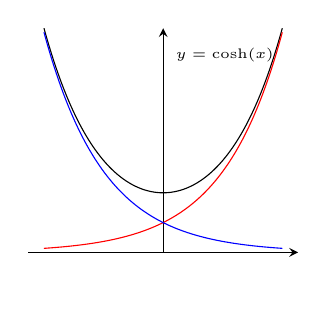
\begin{tikzpicture}
  \begin{axis}[
        axis x line=middle,
      axis y line=middle,
      axis equal,
%       xlabel = {$x$},
%       ylabel = {$y$},
      xtick={\empty},
      ytick={\empty},
      restrict y to domain = -0.5:8,
      restrict x to domain = -2:2,
      scale=0.5
    ]
    \addplot [domain = -2:2, samples = 500,scale=0.2]
      ({x}, {0.5*(exp(x)+exp(-x))});
     \addplot [domain = -2:2, samples = 500,scale=0.2,color=red]
      ({x}, {0.5*exp(x))});
      \addplot [domain = -2:2, samples = 500,scale=0.2,color=blue]
      ({x}, {0.5*exp(-x))});
      \addplot [domain = -2:2, samples = 2,scale=0.2]
      ({x},0);
      

      
  \end{axis};
  
    %\draw[blue] (-0.25,1) node[right] {$\frac{1}{2}e^{-x}$};
    %\draw[red] (2.5,1) node[right] {$\frac{1}{2}e^{x}$};
     %\draw[black] (1,2.5) node[right] {$\frac{e^{x}+e^{-x}}{2}$};
 \draw[black] (1.75,2.5) node[right] {\tiny{$y=\cosh(x)$}};
\draw[red] (2.5,-0.25) node[right] {};
    \end{tikzpicture}



	
\end{document}
